\subsection{In-Depth Analysis}
\label{subsec:in_depth_analysis}

\begin{figure}[t]
    \centering
    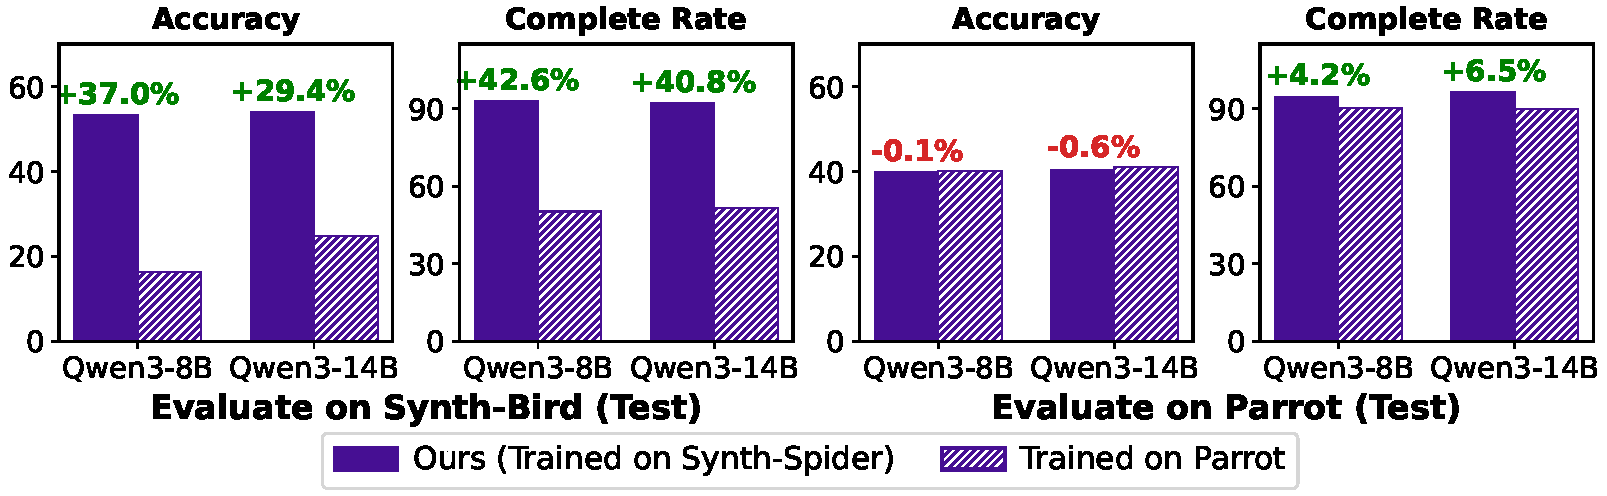
\includegraphics[width=1.01\columnwidth]{plots/plot/trained_on_spider_and_parrot.pdf}
    \vspace{-2em} 
    \caption{Evaluation results of models trained on Synth-Spider (Train) and Parrot (Train).}
    \label{\labelprefix fig:trained_on_spider_and_parrot}
    \vspace{-1em}
\end{figure}
\revise{

\stitle{Exp-\expnum\label{exp:data_effectiveness}: Effectiveness of Synthesized Training Data.}
We evaluate whether models trained on our synthesized Synth-Spider dataset generalize better than those trained on the public Parrot dataset. 
% Both models are evaluated on the Synth-Bird Test set.
We first evaluate these two models on Synth-Bird (Test) under the out-of-domain setting. As illustrated in the left of Figure~\ref{fig:trained_on_spider_and_parrot}, training on Synth-Spider yields much higher performance: accuracy increases by 37.0 and 29.4 points on Qwen3-8B and Qwen3-14B over Parrot. 
% Completion rate shows even larger gains, with increases of 42.6 and 40.8 respectively.
To further highlight the effectiveness of synthesized data, we adopt a more challenging setting. We evaluate models trained on Synth-Spider under a totally out-of-domain setting and models trained on Parrot under an in-domain setting on Parrot (Test), as illustrated in the right of Figure~\ref{fig:trained_on_spider_and_parrot}. Our synthesized data are still competitive under such a challenging experimental setting. Models trained on Synth-Spider achieve accuracy comparable to models trained on Parrot (40.44 vs. 40.99 on Qwen3-8B).

\begin{shaded}
\noindent \textbf{Finding \findingnum: 
Our synthetic training data provides effective supervision for agentic training, significantly improving the performance on unseen tasks.
}
\end{shaded}
}



\revise{
\begin{table}[t]
  \centering
  \caption{\bf Results on the Buildings dataset (real-world).}
  \vspace{-1em}
  \label{\labelprefix tbl:buildings_exp}
  \resizebox{0.68\columnwidth}{!}{
    \begin{tabular}{|c||c|c|c|}
      \hline
      \textbf{Method} & \textbf{Acc.} & \textbf{Comp.} & \textbf{Cost (\$)} \\
      \hline \hline
      % CodeGen & 71.43 & 95.24\% & \textbf{0.0017} \\
      ReAct & 74.29 & 99.05\% & \textbf{0.0052} \\
      CodeGen & 71.43 & 100\% & 0.0054 \\
      MontePrep & 72.38 & 86.67\% & 0.043 \\
      MCTS-OP & 69.52 & 99.05\% & 0.057 \\
      \hline \hline
      \textbf{\sys (Ours)} & \textbf{82.85} & \textbf{100\%} & {0.0082} \\
      \hline
    \end{tabular}
  }
  \vspace{-1em}
\end{table}


\stitle{Exp-\expnum\label{exp:building_exp}: Generalization on Real-World Dataset.}
We have compared \sys with prompting baselines on the real-world dataset Buildings~\cite{sharma2023automatic}. Table~\ref{\labelprefix tbl:buildings_exp} reports Accuracy, Completion Rate and API Cost per case. As illustrated, \sys generalizes well on the real-world dataset. Specifically, \sys achieves the best Accuracy of 82.85 and maintains relatively low inference
cost (0.008\$ per case). This enhances its usability in real-world.

\stitle{Error Analysis.} We further conduct an error analysis of this experiment and identify two key challenges in real-world scenarios. (1) Real cases often contain abbreviated or domain-specific column names, leading to selecting the wrong columns required to be mapped into the target columns. (2) The target specification in real cases is often under-specified. For example, whether daily or monthly granularity is expected is not specified clearly in the requirement. We will address these challenges in our future work. The complete statistics can be found in our technical report~\cite{technical_report}.

\begin{shaded}
\noindent
\textbf{Finding \findingnum: \sys generalizes well to the real-world Buildings dataset.}
\end{shaded}}

\revise{

\begin{figure}[t]
    \centering
    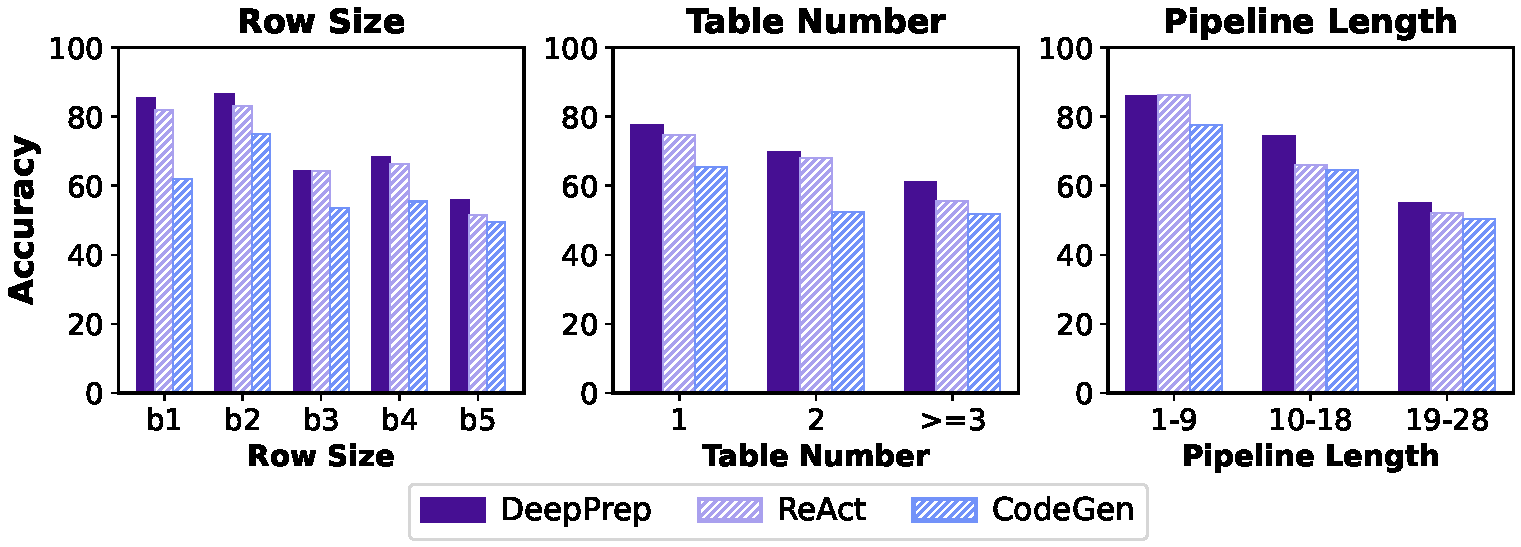
\includegraphics[width=0.99\columnwidth]{figures/fig/overview_synth_spider.pdf}
    \vspace{-1em}
    \caption{Scalability analysis on Synth-Spider with varying (a) row size, (b) source table number, and (c) pipeline length.}
    \label{fig:scalability_synth_spider}
    \vspace{-1em}
\end{figure}


\stitle{Exp-\expnum\label{exp:scalability}: Scalability Analysis.}
We evaluate the scalability of \sys on Synth-Spider from three dimensions: row size, number of source tables, and pipeline length.
% and report the accuracy results, time usage and resource usage. 

\stitle{Scalability Analysis of Accuracy.} As shown in Figure~\ref{fig:scalability_synth_spider}(a), \sys remains robust on small and medium-sized tables. Performance degrades only for the largest row-size bucket ($b_5$: 36 to 124k+ rows), where accuracy decreases by 29.54 points compared with the smallest bucket ($b_1$: 1 to 9 rows). This degradation is primarily caused by the table sampling strategy used to control token usage, where relevant information may be omitted from the sampled content. As shown in Figure~\ref{fig:scalability_synth_spider}, performance decreases as more source tables are involved, but \sys consistently achieves the highest accuracy across different table number groups. As illustrated, all methods degrade as the pipeline length increases.
% , reflecting the greater difficulty of long-horizon pipeline construction. 
However, \sys shows the smallest degradation, and its advantage over baselines becomes larger on complex cases. 

\stitle{Scalability Analysis of Time and Resource Usage.} \sys exhibits stable growth in both execution time and memory usage as workload complexity increases. For example, on Synth-Spider, the average execution time increases only from 8.91 to 11.30 seconds when moving from the smallest to the largest column-size bucket, while memory usage remains between 66 MB and 69 MB. The stable scaling behavior can be explained by the generative search framework, as defined in Section~\ref{sec:tree_based_agentic_reasoning}. The process is bounded by the maximum exploration turn $T$ and the maximum operator sequence length $L$ per expansion, yielding a worst-case complexity of $O(T\times L)$. Unlike MCTS-based methods, \sys generates only one operator pipeline conditioned on the current tree state. The ``pruning'' is implicit in the LLM’s decision-making. Consequently, the effective branching factor depends on the LLM’s learned policy and remains bounded regardless of input size, which explains the stable growth in time and memory usage.

Complete scalability results across all datasets and detailed time and resource usage analysis are provided in our technical report~\cite{technical_report}.

\begin{shaded}
\noindent
\textbf{Finding \findingnum: \sys maintains robust accuracy and stable resource usage as workload complexity increases.}
\end{shaded}

}

